\documentclass[semifinal]{cpecmu}

%% This is a sample document demonstrating how to use the CPECMU
%% project template. If you are having trouble, see "cpecmu.pdf" for
%% documentation.

\projectNo{S007-1}
\acadyear{2025}

\titleTH{GymMate : เพื่อนรู้ใจเรื่องฟิตเนส}
\titleEN{GymMate : Your Fitness Buddy}

\author{ภาณุเดช เสือเผือก}{Phanudet Sueaphueak}{650610797}
\author{ภูเบศร์ เรืองคุ้ม}{Pubest Ruengkum}{650610798}
\author{อนวัช รัตนกิจศร}{Anawat Rattanakitsorn}{650610818}

\cpeadvisor{navadon}
\cpecommittee{dome}
\cpecommittee{lachana}

%\committee{รศ.ดร.\,นิพนธ์ ธีรอำพน}{Assoc.\,Prof.\,Nipon Theera-Umpon, Ph.D.}

%% Some possible packages to include:
\usepackage[final]{graphicx} % for including graphics
\usepackage{booktabs} 
%% Add bookmarks and hyperlinks in the document.
\PassOptionsToPackage{hyphens}{url}
\usepackage[colorlinks=true,allcolors=Blue4,citecolor=red,linktoc=all]{hyperref}
\def\UrlLeft#1\UrlRight{$#1$}

%% Needed just by this example, but maybe not by most reports
\usepackage{afterpage} % for outputting
\usepackage{pdflscape} % for landscape figures and tables. 

%% Some other useful packages. Look these up to find out how to use
%% them.
% \usepackage{natbib}    % for author-year citation styles
% \usepackage{txfonts}
% \usepackage{appendix}  % for appendices on a per-chapter basis
% \usepackage{xtab}      % for tables that go over multiple pages
% \usepackage{subfigure} % for subfigures within a figure
% \usepackage{pstricks,pdftricks} % for access to special PostScript and PDF commands
% \usepackage{nomencl}   % if you have a list of abbreviations

%% if you're having problems with overfull boxes, you may need to increase
%% the tolerance to 9999
% \tolerance=9999

\bibliographystyle{plain}
% \bibliographystyle{IEEEbib}

% \renewcommand{\topfraction}{0.85}
% \renewcommand{\textfraction}{0.1}
% \renewcommand{\floatpagefraction}{0.75}

%% Example for glossary entry
%% Need to use glossary option
%% See glossaries package for complete documentation.
\ifglossary
  \newglossaryentry{lorem ipsum}{
    name=lorem ipsum,
    description={derived from Latin dolorem ipsum, translated as ``pain itself''}
  }
\fi

%% Uncomment this command to preview only specified LaTeX file(s)
%% imported with \include command below.
%% Any other file imported via \include but not specified here will not
%% be previewed.
%% Useful if your report is large, as you might not want to build
%% the entire file when editing a certain part of your report.
% \includeonly{chapters/intro,chapters/background}

\begin{document}
\maketitle
\makesignature

\ifproject
\begin{abstractTH}
\enskip ปัจจุบันผู้ใช้บริการฟิตเนส โดยเฉพาะผู้เริ่มต้น มักประสบปัญหาขาดความรู้ในการออกกำลังกาย ขาดแรงจูงใจ และไม่มีระบบติดตามความก้าวหน้า ขณะเดียวกันผู้ประกอบการฟิตเนสยังขาดเครื่องมือดิจิทัลที่ช่วยบริหารจัดการเครื่องเล่นและสร้างการมีส่วนร่วมกับสมาชิก โครงงานนี้มีวัตถุประสงค์เพื่อสำรวจและออกแบบระบบ GymMate ซึ่งเป็นแพลตฟอร์มในรูปแบบ Web/Mobile Application ที่ผสานแนวคิด Gamification เข้ากับ Workout Recommendation และ Program Planner ระบบที่ออกแบบมีฟังก์ชันสำคัญ ได้แก่ โปรแกรมการฝึก (ทั้งแบบสำเร็จรูปและแบบปรับแต่งได้), การแสดงแผนผังยิม (Floorplan) พร้อมปุ่ม Flex Substitute เพื่อแนะนำเครื่องหรือท่าทางทดแทนเมื่ออุปกรณ์ไม่ว่าง, ระบบบันทึกและวิเคราะห์ความก้าวหน้า, การสะสมคะแนนและจัดอันดับเพื่อสร้างแรงจูงใจ รวมถึงแดชบอร์ดสำหรับผู้ดูแลในการจัดการข้อมูลเครื่องเล่นและพื้นที่ยิม ผลลัพธ์ของโครงงานนี้คือชุดคุณลักษณะและต้นแบบ UX/UI ที่ผ่านการเก็บและวิเคราะห์ความต้องการจากอาจารย์ที่ปรึกษา เจ้าของยิม และผู้จัดการฟิตเนส โดยอ้างอิงมาตรฐาน ACSM Guidelines และ Physical Activity Guidelines เพื่อนำไปสู่การพัฒนาระบบต้นแบบที่สามารถสนับสนุนการออกกำลังกายอย่างมีประสิทธิภาพและยั่งยืนได้ในอนาคต
\end{abstractTH}



\begin{abstract}
Fitness users, especially beginners, often face challenges such as a lack of exercise knowledge, insufficient motivation, and the absence of effective progress-tracking tools. At the same time, gym owners lack digital solutions to manage equipment efficiently and engage members. This project aims to survey and design GymMate, a Web/Mobile application platform that integrates Gamification with Workout Recommendation and Program Planning. The proposed system includes key features such as preset and customizable workout programs, an interactive Gym Floorplan with a Flex Substitute function to suggest alternative machines or exercises when equipment is occupied, progress tracking and analytics, gamification elements (points, badges, streaks, and leaderboards), and an admin dashboard for managing gym equipment and information. The outcome of this project is a refined set of features and UX/UI prototypes, derived through iterative requirement gathering with advisors, gym owners, and fitness managers. The design also references the ACSM Guidelines and Physical Activity Guidelines, laying the foundation for a future prototype that supports effective and sustainable fitness training.
\end{abstract}

\iffalse
\begin{dedication}
This document is dedicated to all Chiang Mai University students.

Dedication page is optional.
\end{dedication}
\fi % \iffalse

\begin{acknowledgments}
โครงงาน \textbf{GymMate : เพื่อนรู้ใจเรื่องฟิตเนส (GymMate : Your Fitness Buddy)} ไม่อาจสำเร็จลุล่วงได้ หากปราศจากแรงสนับสนุน คำแนะนำ และความช่วยเหลือจากหลายฝ่าย คณะผู้จัดทำขอถือโอกาสนี้แสดงความขอบคุณอย่างจริงใจต่อทุกท่านที่มีส่วนร่วมในการผลักดันให้โครงงานนี้สำเร็จลุล่วง

คณะผู้จัดทำขอขอบคุณ \textbf{ผู้ช่วยศาสตราจารย์ ดร.\ นวดนย์ คุณเลิศกิจ} อาจารย์ที่ปรึกษาโครงงาน ที่ได้ให้คำแนะนำทั้งด้านวิชาการและแนวทางการพัฒนาอย่างต่อเนื่องตลอดระยะเวลาของโครงงาน นอกจากนี้ขอขอบคุณ \textbf{ผู้ช่วยศาสตราจารย์ โดม โพธิกานนท์} และ \textbf{ผู้ช่วยศาสตราจารย์ ดร.\ ลัชนา ระมิงค์วงศ์} อาจารย์กรรมการสอบโครงงาน ที่ได้สละเวลาตรวจสอบและให้ข้อเสนอแนะอันมีค่า

คณะผู้จัดทำขอขอบคุณ \textbf{ภาควิชาวิศวกรรมคอมพิวเตอร์ คณะวิศวกรรมศาสตร์ มหาวิทยาลัยเชียงใหม่} ที่ให้การสนับสนุนด้านทรัพยากรและองค์ความรู้ รวมถึงผู้เข้าร่วมทดสอบการใช้งานระบบ (Usability Testing) ทุกท่าน ที่ให้ข้อเสนอแนะอันเป็นประโยชน์ต่อการพัฒนาระบบ สุดท้ายขอขอบคุณครอบครัวทุกท่านที่ให้การสนับสนุนและเป็นกำลังใจตลอดมา

\acksign{2026}{3}{24}
\end{acknowledgments}
\fi % \ifproject

\contentspage

\ifproject
\figurelistpage

\tablelistpage
\fi % \ifproject

% \abbrlist % this page is optional

% \symlist % this page is optional

% \preface % this section is optional


\pagestyle{empty}\cleardoublepage
\normalspacing \setcounter{page}{1} \pagenumbering{arabic} \pagestyle{cpecmu}

\chapter{\ifenglish Introduction\else บทนำ\fi}

\section{\ifenglish Project rationale\else ที่มาของโครงงาน\fi}
\enskip ปัจจุบันมีการส่งเสริมให้นักศึกษามหาวิทยาลัยเชียงใหม่หันมาใส่ใจสุขภาพและการออกกำลังกายมากขึ้น \\โดยมีบริการฟิตเนสภายในมหาวิทยาลัย เช่น CMU Fitness by Playground อย่างไรก็ตาม พบว่าผู้ใช้งานจำนวนไม่น้อยยังประสบปัญหาขาดแรงจูงใจ ความต่อเนื่องในการออกกำลังกาย รวมถึงความยุ่งยากในการวางแผนการฝึกและการเลือกใช้อุปกรณ์อย่างเหมาะสม

\enskip จากสภาพปัญหาดังกล่าว จึงเกิดแนวคิดในการพัฒนาโครงงาน GymMate ซึ่งมีจุดมุ่งหมายเพื่อเป็นต้นแบบระบบที่ช่วยสนับสนุนการออกกำลังกายของนักศึกษา โดยเน้นการสร้างแรงจูงใจและการจัดการการใช้งานฟิตเนสให้มีประสิทธิภาพมากยิ่งขึ้น

\section{\ifenglish Objectives\else วัตถุประสงค์ของโครงงาน\fi}
\setlength{\leftmargini}{1.25cm}
\begin{enumerate}
\renewcommand{\labelenumi}{1.2.\arabic{enumi}}
    \item พัฒนาระบบการวางแผนการออกกำลังกาย (Workout Program Planner)\\
    GymMate มุ่งเน้นการพัฒนาโปรแกรมฝึกที่สามารถเลือกได้ทั้งรูปแบบสำเร็จรูป (preset) และการปรับแต่งตามความต้องการ (custom) เพื่อช่วยให้นักศึกษาสามารถวางแผนการออกกำลังกาย\\ได้สะดวกและเหมาะสมกับเป้าหมายของตนเอง

    \item เพิ่มประสิทธิภาพการออกกำลังกายด้วยระบบ Flex Substitute\\
    ด้วยระบบแนะนำท่าและเครื่องเล่นทดแทนอัตโนมัติ เมื่ออุปกรณ์ที่ต้องการไม่พร้อมใช้งาน ผู้ใช้สามารถเลือกทางเลือกที่เหมาะสมกับกล้ามเนื้อที่ต้องการฝึกได้ โดยระบบจะช่วยแนะนำผ่านอัลกอริทึมที่ออกแบบมาโดยเฉพาะ

    \item จัดการฟิตเนสอย่างเป็นระบบผ่าน CMS Dashboard\\
    ฝั่งผู้ดูแลฟิตเนสสามารถจัดการตำแหน่งและข้อมูลเครื่องเล่นได้อย่างมีประสิทธิภาพ \\ลดความซับซ้อนในการบริหารจัดการ และเพิ่มความสะดวกให้กับทั้งผู้ดูแลและผู้ใช้งาน

    \item สร้างแรงจูงใจและความต่อเนื่องในการออกกำลังกาย\\
    ด้วยระบบ Gamification และ Leaderboard ผู้ใช้งานสามารถสะสมคะแนน แข่งขันกับผู้ใช้คนอื่น ติดตามความก้าวหน้าของตนเอง ทำให้การออกกำลังกายน่าสนใจ สนุก และมีแรงกระตุ้นมากขึ้น
\end{enumerate}

\section{\ifenglish Project scope\else ขอบเขตของโครงงาน\fi}
\enskip โครงงาน GymMate มีขอบเขตการดำเนินงานที่เน้นการ สำรวจและออกแบบระบบต้นแบบ โดยมีรายละเอียดดังนี้

\subsection{\ifenglish  Target Users\else กลุ่มเป้าหมาย\fi}
\begin{itemize}
    \item \textbf{ผู้ใช้บริการฟิตเนส (Fitness Members):}\\
    โดยเฉพาะกลุ่มผู้เริ่มต้น (Beginners) และนักศึกษามหาวิทยาลัยเชียงใหม่ ที่ต้องการโปรแกรมฝึก การติดตามความก้าวหน้า และแรงจูงใจในการออกกำลังกาย
    \item \textbf{ผู้จัดการและเจ้าของฟิตเนส (Gym Managers \&  Owners):}\\
    ต้องการเครื่องมือในการบริหารจัดการเครื่องเล่นและสื่อสารกับสมาชิก เพื่อเพิ่มประสิทธิภาพการใช้งานพื้นที่และเสริมความพึงพอใจของลูกค้า
\end{itemize}

\subsection{\ifenglish  System Features in Scope\else ขอบเขตฟังก์ชัน\fi}
\begin{enumerate}
    \item \textbf{Workout Program Planner} ระบบวางแผนโปรแกรมการออกกำลังกาย\\
    ผู้เริ่มต้นสามารถเลือกใช้ Preset Plan เพื่อสร้างพื้นฐานการฝึกอย่างเป็นระบบ หรือปรับเป็น Custom Plan ให้สอดคล้องกับเป้าหมายเฉพาะบุคคล พร้อมแนวทาง Goal \& Approach เช่น Push–Pull–Legs, Upper–Lower หรือ Total Body เพื่อเพิ่มประสิทธิภาพ
    \item \textbf{Floorplan UI \& Flex Substitute} ส่วนติดต่อผู้ใช้สำหรับผังพื้นที่และการปรับเปลี่ยนแบบยืดหยุ่น\\
    ระบบมีการจัดทำ แผนผังยิม เพื่อแสดงตำแหน่งและการจัดวางของเครื่องเล่นอย่างชัดเจน อีกทั้งมีฟังก์ชัน ปุ่ม Flex Substitute ที่ช่วยแนะนำเครื่องหรือท่าทางทดแทนเมื่ออุปกรณ์ที่ต้องการใช้งานเต็ม โดยยังคงมุ่งเน้นการฝึกที่กล้ามเนื้อเป้าหมายเดิมเพื่อไม่ให้ผลลัพธ์การออกกำลังกายคลาดเคลื่อน.
    \item \textbf{User Management \& Tracking} ระบบจัดการและติดตามผู้ใช้งาน\\
    ระบบมี โปรไฟล์ผู้ใช้ สำหรับจัดเก็บข้อมูลการฝึก พร้อมการบันทึกสถิติ เช่น จำนวนเซต, ครั้งทำซ้ำ และน้ำหนักที่ใช้ นอกจากนี้ยังมี กราฟความก้าวหน้า เพื่อสะท้อนพัฒนาการอย่างต่อเนื่อง รวมถึงรายงานผลการฝึกในรูปแบบรายสัปดาห์และรายเดือน เพื่อช่วยประเมินและปรับแผนการออกกำลังกายได้อย่างเป็นระบบ
    \item \textbf{Gamification Layer} ชั้นการใช้องค์ประกอบเชิงเกม\\
    ระบบมีการสะสมคะแนนจากความสม่ำเสมอในการฝึก พร้อมกลไกสร้างแรงจูงใจผ่าน Badge, Level, Streak และ Leaderboard ซึ่งช่วยเสริมทั้งความต่อเนื่องและการแข่งขันเชิงบวกระหว่างผู้ใช้
    \item \textbf{Content \& Notification} ระบบจัดการเนื้อหาและการแจ้งเตือน\\
    ระบบรองรับ วิดีโอและภาพประกอบท่าทาง ผ่าน QR code ที่ติดไว้บนเครื่องออกกำลังกาย เพื่อให้ผู้ใช้เข้าถึงวิธีการใช้งานได้อย่างถูกต้อง นอกจากนี้ยังมี การแจ้งเตือน (Notification) ตามตารางโปรแกรม รวมถึงการเปลี่ยนท่าอัตโนมัติเมื่อเครื่องที่ต้องการใช้งานเต็ม เพื่อคงประสิทธิภาพของการฝึก
    \item \textbf{Admin Dashboard (CMS)} แดชบอร์ดผู้ดูแลระบบ\\
    ระบบสามารถ จัดการข้อมูลเครื่องเล่น ได้อย่างยืดหยุ่น ทั้งการเพิ่ม ย้าย หรือแก้ไขสถานะของเครื่องออกกำลังกาย พร้อมทั้งแสดง ข้อมูลพื้นฐานของฟิตเนส เช่น เวลาเปิด–ปิด และข่าวสารที่เกี่ยวข้อง เพื่ออำนวยความสะดวกแก่ผู้ใช้
\end{enumerate}

\subsection{\ifenglish Hardware scope\else ขอบเขตด้านฮาร์ดแวร์\fi}
\enskip โครงงานนี้ไม่ได้พัฒนาฮาร์ดแวร์ใหม่ แต่ใช้โครงสร้างพื้นฐานและบริการที่มีอยู่ ได้แก่
\begin{itemize}
    \item สมาร์ทโฟนของผู้ใช้งานสำหรับติดตั้งและใช้งานแอปพลิเคชัน
    \item สถานที่และเครื่องเล่นออกกำลังกายของยิม
\end{itemize}

\subsection{\ifenglish Software scope\else ขอบเขตด้านซอฟต์แวร์\fi}
\enskip ขอบเขตด้านซอฟต์แวร์ของโครงงานประกอบด้วย
\begin{itemize}
    \item ต้องรองรับการใช้งานและติดตั้งแอปพลิเคชันบนสมาร์ทโฟนของผู้ใช้
    \item ต้องรองรับการใช้งานผ่านคอมพิวเตอร์สำหรับการจัดการ CMS Dashboard ของผู้ดูแลระบบ
\end{itemize}


\section{\ifenglish Expected outcomes\else ประโยชน์ที่ได้รับ\fi}
\setlength{\leftmargini}{1.25cm}
\begin{enumerate}
\renewcommand{\labelenumi}{1.4.\arabic{enumi}}
    \item ได้ต้นแบบแอปพลิเคชัน GymMate ที่ช่วยสนับสนุนการออกกำลังกายและเพิ่มแรงจูงใจสำหรับนักศึกษามหาวิทยาลัยเชียงใหม่
    \item ผู้ใช้งานสามารถวางแผนโปรแกรมการออกกำลังกายได้สะดวกและเหมาะสมกับเป้าหมายของตนเอง ทั้งแบบสำเร็จรูปและแบบปรับแต่ง
    \item ผู้ดูแลฟิตเนสสามารถบริหารจัดการตำแหน่งและข้อมูลเครื่องเล่นได้ง่ายขึ้น ผ่าน CMS Dashboard
    \item ระบบช่วยเพิ่มความต่อเนื่อง สนุก และประสิทธิภาพในการออกกำลังกายของนักศึกษา
    \item โครงงานสามารถต่อยอดไปสู่การใช้งานจริง และขยายผลสำหรับฟิตเนสหรือมหาวิทยาลัยอื่นได้
\end{enumerate}

\section{\ifenglish Technology and tools\else เทคโนโลยีและเครื่องมือที่ใช้\fi}
\enskip เพื่อพัฒนาและนำเสนอระบบ GymMate ได้ตามเป้าหมาย โครงงานนี้เลือกใช้เทคโนโลยีหลัก 3 ส่วน ดังนี้

\begin{enumerate}
\renewcommand{\labelenumi}{1.5.\arabic{enumi}}
    \item \textbf{Web Application (CMS Dashboard)}\\
    ระบบสำหรับ ผู้ดูแล (Admin/Gym Manager) ทำหน้าที่บริหารจัดการข้อมูลเครื่องเล่น รวมถึงการย้ายหรือแก้ไขสถานะใน Floorplan และจัดการข้อมูลฟิตเนส เช่น ข่าวสารและเวลาเปิด–ปิด เพื่อให้การดำเนินงานเป็นระเบียบและมีประสิทธิภาพ
    \item \textbf{Mobile Application (User App)}\\
    ระบบสำหรับ ผู้ใช้ฟิตเนส (Members) รองรับการเลือกโปรแกรมฝึกที่เหมาะสม \\พร้อมฟังก์ชัน Calendar/Day Plan เพื่อดูตารางการฝึก และ Floorplan Highlight ช่วยระบุตำแหน่งเครื่องเล่น นอกจากนี้ยังมี Flex Substitute สำหรับแนะนำท่าทางทดแทน, Log Progress เพื่อบันทึกผลการฝึก, ระบบ Gamification เพื่อสร้างแรงจูงใจ และ Notification สำหรับแจ้งเตือนตามโปรแกรมอย่างต่อเนื่อง
    \item \textbf{Server \& Backend Services}\\
    ระบบนี้ใช้สำหรับ ประมวลผลและจัดเก็บข้อมูล ที่เกี่ยวข้องกับโปรแกรมการฝึก การใช้งาน และการจัดการเครื่อง โดยมีฟังก์ชันหลัก ได้แก่ Workout Planner สำหรับวางแผนการฝึก, Flex Substitute Algorithm เพื่อแนะนำทางเลือกเมื่อเครื่องเต็ม, ระบบ Authentication/Authorization เพื่อควบคุมสิทธิ์การใช้งาน และ Data Logging สำหรับเก็บบันทึกข้อมูลอย่างเป็นระบบ
\end{enumerate}

\section{\ifenglish Project plan\else แผนการดำเนินงาน\fi}

\begin{plan}{6}{2025}{3}{2026}
    \planitem{6}{2025}{7}{2025}{ศึกษาค้นคว้าและหาหัวข้อสําหรับโครงงาน}
    \planitem{7}{2025}{9}{2025}{เก็บและวิเคราะห์ความต้องการ}
    \planitem{8}{2025}{9}{2025}{ออกแบบฟีเจอร์และปรับขอบเขต}
    \planitem{9}{2025}{11}{2025}{ออกแบบ UX/UI และต้นแบบ}
    \planitem{11}{2025}{12}{2025}{ออกแบบเชิงเทคนิค: Database, API, System Architecture}
    \planitem{12}{2025}{2}{2026}{พัฒนา Backend}
    \planitem{1}{2026}{2}{2026}{พัฒนา Mobile App}
    \planitem{1}{2026}{2}{2026}{พัฒนา Web CMS (Admin Dashboard, Floorplan Editor)}
    \planitem{2}{2026}{3}{2026}{ทดลองใช้งานจริงกับผู้ใช้}
\end{plan}

\section{\ifenglish Roles and responsibilities\else บทบาทและความรับผิดชอบ\fi}
\begin{enumerate}
    \item นายภาณุเดช เสือเผือก รับบทบาท Product Owner, Frontend
    \begin{itemize}
        \item \textbf{หน้าที่:} เสนอไอเดียจากประสบการณ์การเข้ายิม, พัฒนา Mobile/Web Frontend, ตรวจสอบความถูกต้องของข้อมูลการออกกำลังกาย
        \item \textbf{ความรู้ที่ใช้:} ความรู้ด้านการออกกำลังกาย และการพัฒนาส่วนติดต่อผู้ใช้ (Frontend Development)
    \end{itemize}

    \item นายภูเบศร์ เรืองคุ้ม รับบทบาท Backend \& System
    \begin{itemize}
        \item \textbf{หน้าที่:} ออกแบบสถาปัตยกรรมระบบและฐานข้อมูล, พัฒนา API และ Flex Substitute และความปลอดภัยระบบ
        \item \textbf{ความรู้ที่ใช้:} การเขียนโปรแกรมฝั่งเซิร์ฟเวอร์ (Backend Programming), ฐานข้อมูล และความปลอดภัยของระบบ
    \end{itemize}
    
    \item นายอนวัช รัตนกิจศร รับบทบาท UX/UI \& Documentation
    \begin{itemize}
        \item \textbf{หน้าที่:} ออกแบบ UX/UI Mockup, จัดทำเอกสารรายงาน, ประสานงานกับอาจารย์และ Stakeholder, สนับสนุนงาน Frontend
        \item \textbf{ความรู้ที่ใช้:} การออกแบบประสบการณ์ผู้ใช้และส่วนติดต่อผู้ใช้ (UX/UI Design), การเขียนเชิงเทคนิค (Technical Writing), การสื่อสาร (Communication)
    \end{itemize}
    
\end{enumerate}

\section{\ifenglish%
Impacts of this project on society, health, safety, legal, and cultural issues
\else%
ผลกระทบด้านสังคม สุขภาพ ความปลอดภัย กฎหมาย และวัฒนธรรม
\fi}

\enskip โครงงาน GymMate อาจมีผลกระทบและการประยุกต์ใช้งานในหลายมิติ ดังนี้

\begin{enumerate}
    \item \textbf{ด้านสังคม:} สนับสนุนให้นักศึกษาหันมาออกกำลังกายมากขึ้น 
    ช่วยสร้างแรงจูงใจผ่านระบบ Gamification และ Leaderboard
    \item \textbf{ด้านสุขภาพ:} ช่วยส่งเสริมสุขภาพกายและจิตใจของผู้ใช้ 
    ลดความเสี่ยงจากโรคที่เกิดจากการขาดการออกกำลังกาย
    \item \textbf{ด้านความปลอดภัย:} การแนะนำการใช้อุปกรณ์และท่าทางอย่างถูกต้อง 
    ลดความเสี่ยงในการบาดเจ็บจากการออกกำลังกาย
    \item \textbf{ด้านกฎหมาย:} ต้องคำนึงถึงลิขสิทธิ์ของข้อมูล รูปภาพ และเพลง 
    รวมถึงการจัดเก็บข้อมูลผู้ใช้ให้เป็นไปตามกฎหมายคุ้มครองข้อมูลส่วนบุคคล (PDPA/GDPR)
    \item \textbf{ด้านวัฒนธรรม:} ปรับการออกแบบแอปให้เหมาะกับวิถีชีวิตและพฤติกรรมของนักศึกษา 
    ส่งเสริมการสร้างวัฒนธรรมการดูแลสุขภาพในมหาวิทยาลัย
\end{enumerate}

%================ Chapter ==================
\chapter{หลักการและทฤษฎีที่เกี่ยวข้อง}
\label{chap:theory}

%================ Section: Scrum Research ==================
\section{กระบวนการรวบรวมและเก็บข้อมูลตามหลัก Scrum}
\label{sec:scrum-research}

\noindent\textbf{วัตถุประสงค์} —
อธิบายแนวทางรวบรวมและตรวจสอบความต้องการภายใต้ Agile/Scrum เพื่อนำผลลัพธ์ไปใช้ต่อในการออกแบบและพัฒนาซอฟต์แวร์

\vspace{0.6em}
\noindent\textbf{ภาพรวมกระบวนการ}
\begin{enumerate}
  \item \textbf{แหล่งข้อมูล}: ใช้วิธีการต่างๆ เพื่อรวบรวมความต้องการ เช่น การสัมภาษณ์, การสังเกตการณ์ผู้ใช้, แบบสอบถาม และการวิเคราะห์ระบบเดิมหรือคู่แข่ง
  \item \textbf{สิ่งส่งมอบของ Scrum}: สร้างเอกสารหลักสำหรับการจัดการโครงการ ได้แก่ วิสัยทัศน์ผลิตภัณฑ์, รายการงานทั้งหมด, เรื่องราวของผู้ใช้, เกณฑ์การยอมรับงาน และข้อกำหนดว่าอะไรพร้อมทำงานหรืออะไรเสร็จสมบูรณ์แล้ว
  \item \textbf{รูปแบบ User Story}: เขียนความต้องการในมุมมองผู้ใช้ โดยใช้โครงสร้าง:
    \begin{quote}
      ในฐานะ \textit{[บทบาท]} \\
      ฉันต้องการ \textit{[ความสามารถ]} \\
      เพื่อที่จะ \textit{[ได้รับประโยชน์]}
    \end{quote}
  \item \textbf{การปรับแต่งแบ็กล็อก}: จัดการรายการงานโดยการจัดลำดับความสำคัญ, แบ่งงานใหญ่ให้เป็นงานย่อยที่จัดการได้ และเพิ่มรายละเอียดเงื่อนไขการยอมรับงาน
  \item \textbf{จังหวะการทำงาน}: ดำเนินงานเป็นวงจรซ้ำๆ เริ่มจากขั้นวางแผน 
    $\rightarrow$ พัฒนา $\rightarrow$ นำเสนอผลงาน $\rightarrow$ 
    เรียนรู้และปรับปรุง เพื่อพัฒนาความต้องการอย่างต่อเนื่อง
\end{enumerate}

\begin{figure}[h]
  \centering
  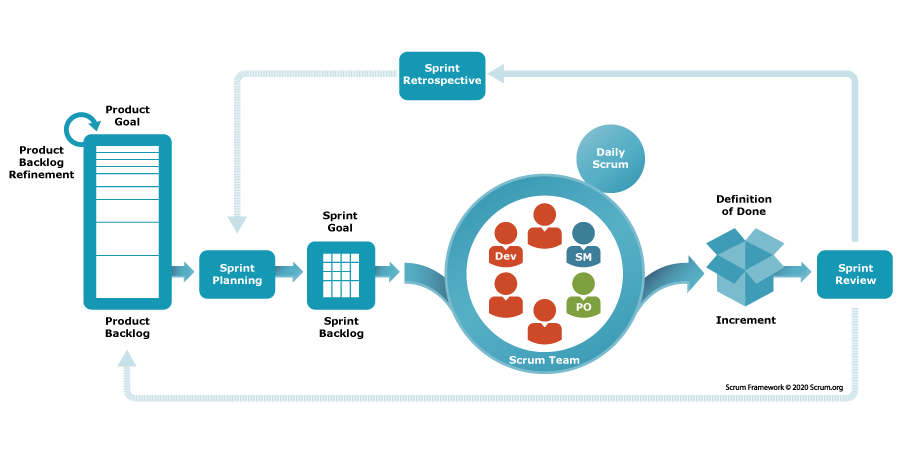
\includegraphics[width=.92\linewidth]{chapters/Images/SCRUM.png}
  \caption{แผนภาพแสดงหลักการพัฒนาซอฟต์แวร์แบบ Scrum}
  \label{fig:scrum-data-flow}
\end{figure}

%================ Section: DB Normalization & Index ==================
\section{หลักการออกแบบฐานข้อมูลโดยอิงตามหลัก Normal Form และ Index เพื่อประสิทธิภาพ}
\label{sec:db-normal-index}

\noindent
การออกแบบข้อมูลประกอบด้วยสองส่วนหลัก: \textbf{ความถูกต้องเชิงตรรกะ} (Normalization) และ \textbf{ประสิทธิภาพการเข้าถึง} (Indexing)

\subsection*{Normalization (1NF–3NF/BCNF)}
\begin{table}[h]
\centering
\begin{tabular}{@{}ll@{}}
\toprule
\textbf{นอร์มอลฟอร์ม} & \textbf{เกณฑ์หลักโดยย่อ} \\
\midrule
1NF & ค่าทุกช่องเป็นอะตอม ไม่มีกลุ่มซ้ำ/ซ้อน \\
2NF & อยู่ใน 1NF และไม่มีการพึ่งพาบางส่วนกับคีย์เชิงประกอบ \\
3NF & อยู่ใน 2NF และไม่มีการพึ่งพาแบบทรานซิทีฟกับคีย์ \\
BCNF & ทุกตัวกำหนด (determinant) ต้องเป็นคีย์แคนดิเดต \\
\bottomrule
\end{tabular}
\caption{สรุป Normal Forms ที่ใช้ในการออกแบบ}
\label{tab:nf}
\end{table}

\subsection*{Indexing เบื้องต้นเพื่อประสิทธิภาพ}
\begin{itemize}
  \item \textbf{ชนิดดัชนี}: B-tree (ทั่วไป/ช่วง), Hash (เท่ากับ), GiST/GIN (JSONB, full-text), BRIN (ตารางใหญ่เรียงตามช่วง)
  \item \textbf{หลักคิด}: เลือกคอลัมน์ที่มี selectivity สูง, ใช้ covering index กับคิวรีที่อ่านบ่อย, ระวังการทำดัชนีมากเกินไป (กระทบงานเขียน)
  \item \textbf{คอมโพสิตอินเด็กซ์}: จัดลำดับคอลัมน์ตาม WHERE/ORDER BY ที่พบบ่อย
\end{itemize}

\noindent\textit{ตัวอย่าง (แนวคิด)}:
\begin{verbatim}
-- คิวรีอ่านบ่อย: recent workouts ของผู้ใช้
CREATE INDEX idx_workout_user_time
ON workout(user_id, started_at DESC);

-- ค้นหา exercise ชื่อแบบ full-text (PostgreSQL)
CREATE INDEX idx_exercise_name_fts
ON exercise USING GIN (to_tsvector('simple', name));
\end{verbatim}

%================ Section: System Architecture ==================
\section{สถาปัตยกรรมของแอพนี้}
\label{sec:system-arch}

\noindent
สถาปัตยกรรมของระบบถูกออกแบบโดยผสมผสาน \textbf{Clean Architecture} สำหรับฝั่ง Backend และโครงสร้างมาตรฐานของ \textbf{Next.js/React Native} สำหรับฝั่ง Frontend เพื่อให้ได้ทั้งความเป็นระเบียบ ความสามารถในการขยาย และการบำรุงรักษาที่ง่ายในอนาคต

\subsection*{โครงสร้างโดยรวม}
\begin{itemize}
  \item \textbf{Client Layer}: 
    \begin{itemize}
      \item \textbf{Web Application} — พัฒนาโดย Next.js (React framework) ใช้โครงสร้างไฟล์มาตรฐาน \texttt{pages/}, \texttt{components/}, \texttt{api/}.
      \item \textbf{Mobile Application} — พัฒนาโดย React Native ตาม format ปกติ (โฟลเดอร์ \texttt{src/}, \texttt{screens/}, \texttt{navigation/}).
      \item รองรับ UI/UX ที่สอดคล้องกับ Figma prototype และมีการเชื่อมต่อ API ผ่าน RESTAPI
    \end{itemize}
  \item \textbf{Backend Layer (Clean Architecture)}:
    \begin{itemize}
      \item \textbf{Domain Layer} — กำหนด business rules, entity, และ interface ที่ไม่ขึ้นกับ framework
      \item \textbf{Use Case Layer} — ตรรกะการทำงาน เช่น การจัดการ workout plan, gamification badge, การวิเคราะห์ข้อมูล
      \item \textbf{Interface Adapter Layer} — แปลงข้อมูลระหว่าง use case/domain กับ external services (เช่น Database, API response)
      \item \textbf{Infrastructure Layer} — เชื่อมต่อกับ Database , Object Storage (ภาพ/วิดีโอ)
    \end{itemize}
  \item \textbf{Data Layer}: 
    \begin{itemize}
      \item ฐานข้อมูลเชิงธุรกรรม (PostgreSQL) สำหรับ core entities (user, workout, program, gamification)
      \item Object storage (เช่น MinIO) สำหรับไฟล์สื่อ เช่น รูป exercise และวิดีโอแนะนำ
    \end{itemize}
\end{itemize}

\subsection*{แนวคิดออกแบบสำคัญ}
\begin{itemize}
  \item \textbf{Separation of Concerns}: Frontend, Backend และ Data Layer ถูกแยกชัดเจน
  \item \textbf{Testability}: Clean Architecture ช่วยให้เขียน unit test ได้ง่าย เนื่องจาก business logic แยกออกจาก framework
  \item \textbf{Scalability}: รองรับการเพิ่มบริการใหม่ เช่น AI-based recommendation หรือ real-time tracking
  \item \textbf{Maintainability}: React/Next และ React Native ใช้ convention เดียวกับ community มาตรฐาน  $\rightarrow$  ลด learning curve สำหรับทีมใหม่
\end{itemize}


%================ Section: Security ==================
\section{หลักการรักษาข้อมูลที่ปลอดภัย}
\label{sec:security}

\noindent
ครอบคลุมความมั่นคงปลอดภัยข้อมูลและการคุ้มครองข้อมูลส่วนบุคคล (purpose limitation, data minimization, storage limitation) และการออกแบบ security by design

\begin{itemize}
  \item \textbf{การระบุตัวตน/การอนุญาต}: MFA, RBAC/ABAC, หลัก least privilege
  \item \textbf{การเข้ารหัส}: in transit (TLS), at rest (TDE/field-level), KMS
  \item \textbf{การเก็บรักษา}: นโยบายตามประเภทข้อมูล; pseudonymization/anonymization
  \item \textbf{การบันทึกเหตุการณ์}: Audit log, tamper-evident, breach notification
  \item \textbf{สิทธิของเจ้าของข้อมูล}: การเข้าถึง/แก้ไข/ลบ/จำกัด/พกพาข้อมูล
\end{itemize}

%================ Section: Health Science ==================
\section{วิทยาศาสตร์ทางด้านสุขภาพ}
\label{sec:health-science}

\noindent
วางรากฐานเชิงวิทยาศาสตร์สำหรับคุณลักษณะของระบบที่เกี่ยวกับการออกกำลังกายและพฤติกรรมผู้ใช้

\subsection{แนวทางของ ACSM (American College of Sports Medicine)}
\label{subsec:acsm}

\noindent
แนวทางจาก \textbf{ACSM} เป็นมาตรฐานสากลสำหรับการสั่งการออกกำลังกาย โดยอ้างอิงหลัก \textbf{FITT-VP} และขยายรายละเอียดสำหรับประชากรทั่วไป ดังนี้:

\begin{itemize}
  \item \textbf{แอโรบิก (Aerobic)}: อย่างน้อย 150 นาที/สัปดาห์ ของการออกกำลังกายระดับปานกลาง (หรือ 75 นาที/สัปดาห์ ของระดับหนัก) กระจาย 3–5 วัน/สัปดาห์
  \item \textbf{การฝึกแรงต้าน (Resistance Training)}: อย่างน้อย 2 วัน/สัปดาห์ ครอบคลุมกล้ามเนื้อหลักทุกมัด 8–12 ครั้ง/ท่า 2–4 เซ็ต
  \item \textbf{การยืดเหยียด (Flexibility)}: อย่างน้อย 2–3 วัน/สัปดาห์ ค้างแต่ละครั้ง 10–30 วินาที 2–4 รอบ
  \item \textbf{การฝึกประสาทและการเคลื่อนไหว (Neuromotor/Functional)}: อย่างน้อย 2–3 วัน/สัปดาห์ เช่น balance, agility, coordination, proprioception
  \item \textbf{หลักการเพิ่มเติม}: 
    \begin{itemize}
      \item ใช้ \%HRmax, \%HRR, RPE หรือ MET เป็นตัวกำหนดความหนัก
      \item ค่อยๆ เพิ่มภาระ (progressive overload) ตามสมรรถภาพและความปลอดภัย
      \item เน้นการออกกำลังกายที่หลากหลาย (multimodal) เพื่อลดการบาดเจ็บและเพิ่ม adherence
    \end{itemize}
\end{itemize}


\chapter{\ifproject%
\ifenglish Project Structure and Methodology\else โครงสร้างและขั้นตอนการทำงาน\fi
\else%
\ifenglish Project Structure\else โครงสร้างของโครงงาน\fi
\fi
}

ในบทนี้จะกล่าวถึงหลักการ และการออกแบบระบบ

\makeatletter

% \renewcommand\section{\@startsection {section}{1}{\z@}%
%                                    {13.5ex \@plus -1ex \@minus -.2ex}%
%                                    {2.3ex \@plus.2ex}%
%                                    {\normalfont\large\bfseries}}

\makeatother
%\vspace{2ex}
% \titleformat{\section}{\normalfont\bfseries}{\thesection}{1em}{}
% \titlespacing*{\section}{0pt}{10ex}{0pt}

\section{โครงสร้างและขั้นตอนการพัฒนา}
\label{sec:development-structure}

\subsection{การวิจัยผู้ใช้และวิเคราะห์ปัญหา (User Research \& Problem Analysis)}
\label{subsec:user-research}

ในขั้นตอนนี้จะมุ่งเน้นการทำความเข้าใจผู้ใช้และปัญหาที่แท้จริงผ่านวิธีการต่างๆ เช่น
\begin{itemize}
    \item การสัมภาษณ์ผู้มีส่วนได้ส่วนเสีย (Stakeholder Interviews)
    \item การสังเกตการณ์และการศึกษาพฤติกรรมผู้ใช้ (User Observation \& Behavior Study)
    \item การวิเคราะห์คู่แข่งและตลาด (Competitor \& Market Analysis)
    \item การระบุ pain points และความต้องการที่แท้จริง (Pain Points \& Real Needs Identification)
\end{itemize}

\subsection{การกำหนดขอบเขตและข้อกำหนด (Scope \& Requirements Definition)}
\label{subsec:requirements-definition}

หลังจากเข้าใจปัญหาแล้ว ขั้นตอนนี้จะเป็นการกำหนดขอบเขตและข้อกำหนดที่ชัดเจน:
\begin{itemize}
    \item การระบุขอบเขตโซลูชัน (Solution Scope)
    \item การจัดลำดับความสำคัญของปัญหา (Problem Prioritization)
    \item การกำหนดข้อกำหนดซอฟต์แวร์ (Software Requirements)
    \item การสร้าง Problem-to-Feature Mapping
\end{itemize}

\begin{figure}[h!]
  \centering
  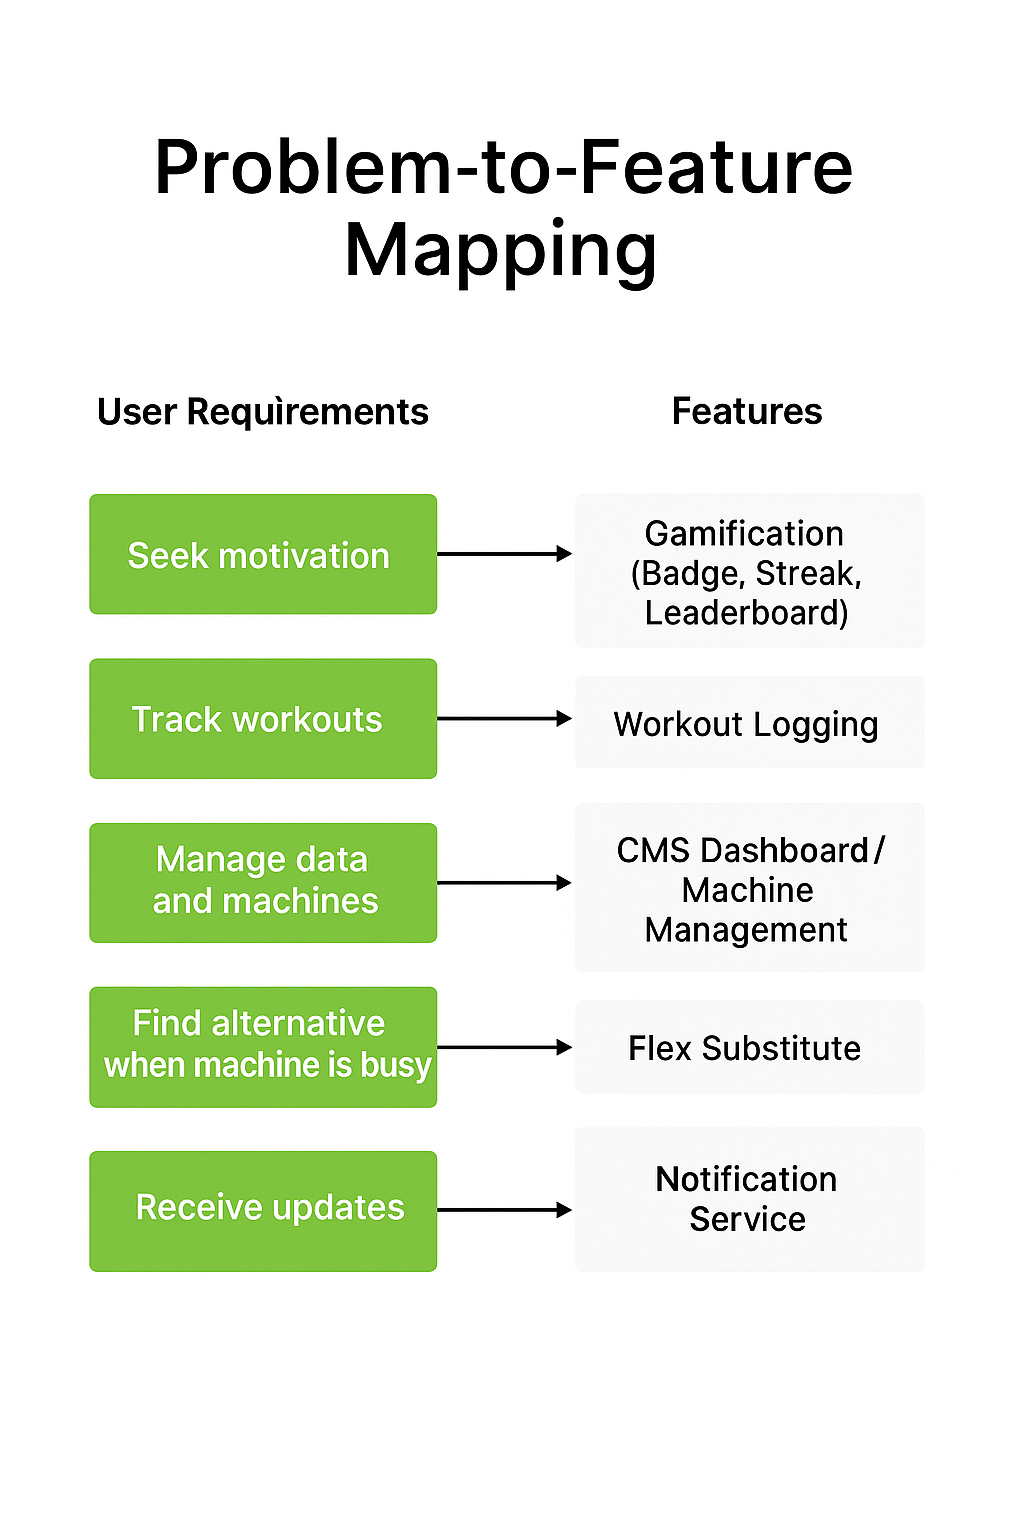
\includegraphics[width=0.35\textwidth]{chapters/Images/Mapping.png}
  \caption{แผนภาพแสดงProblem->Features: กรอบการออกแบบสำหรับ GymMate}
  \label{fig:mapping}
\end{figure}

\subsection{การออกแบบประสบการณ์ผู้ใช้ (User Experience Design)}
\label{subsec:ux-design}

ขั้นตอนการออกแบบประสบการณ์ผู้ใช้ประกอบด้วย:
\begin{itemize}
    \item การกำหนด Use Cases หลัก (Core Use Cases Definition)
    \item การออกแบบ User Flows และเส้นทางผู้ใช้ (User Flows \& Journey Design)
    \item การสร้าง Wireframes และ Prototypes
    \item การทดสอบความใช้งานได้ (Usability Testing)
\end{itemize}
\vspace{1em}

\begin{figure}[h!]
  \centering
  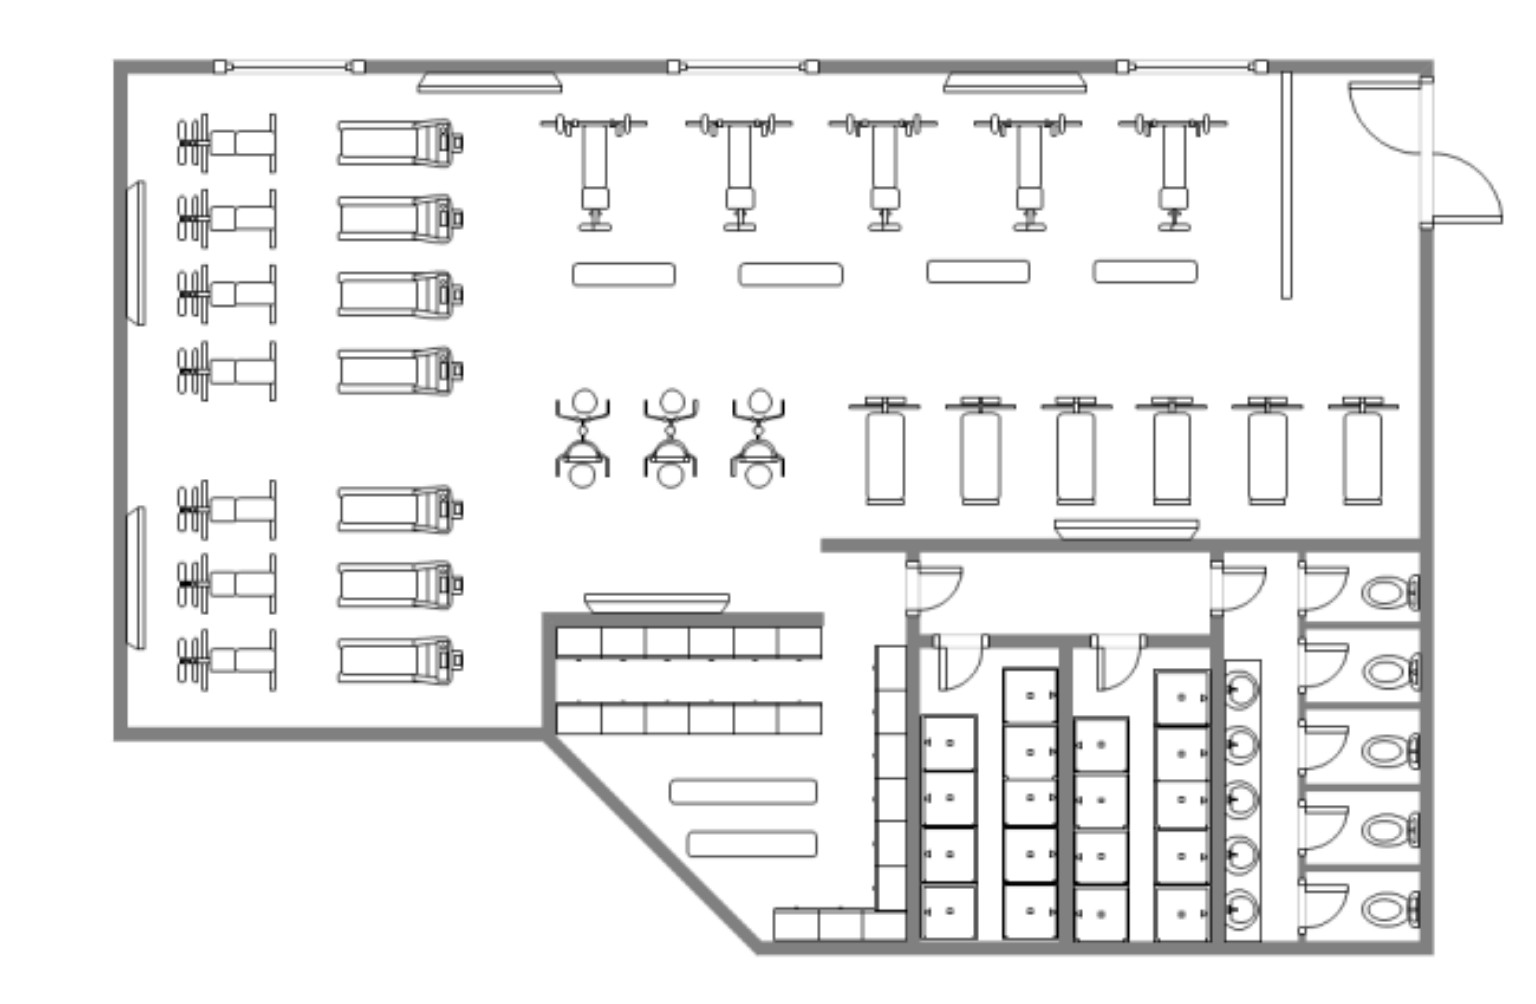
\includegraphics[width=0.35\textwidth]{chapters/Images/Floorplan.png}
  \caption{Simplified Floor Plan of Gym Layout in GymMate}
  \label{fig:floorplan}
\end{figure}

\subsection{การออกแบบระบบและข้อมูล (System \& Data Design)}
\label{subsec:system-design}

การออกแบบด้านเทคนิคของระบบประกอบด้วย:
\begin{itemize}
    \item การออกแบบ Domain Model
    \item การออกแบบโครงสร้างข้อมูล (Data Structure Design)
    \item การออกแบบสถาปัตยกรรมซอฟต์แวร์ (Software Architecture Design)
    \item การออกแบบ API (API Design)
\end{itemize}

\subsection{การออกแบบความปลอดภัยและความเป็นส่วนตัว (Security \& Privacy by Design)}
\label{subsec:security-design}

การออกแบบด้วยแนวคิดความปลอดภัยและความเป็นส่วนตัวตั้งแต่เริ่มต้น:
\begin{itemize}
    \item การวิเคราะห์ความเสี่ยงด้านความปลอดภัย (Security Risk Analysis)
    \item การออกแบบตามหลัก PDPA (PDPA Compliance Design)
    \item การกำหนดนโยบายการเข้าถึงข้อมูล (Data Access Policies)
    \item การป้องกันข้อมูลส่วนบุคคล (Personal Data Protection)
\end{itemize}

\subsection{การออกแบบโครงสร้างพื้นฐานและการส่งมอบ (Infrastructure \& Delivery Design)}
\label{subsec:infrastructure-design}

การออกแบบสภาพแวดล้อมและกระบวนการส่งมอบ:
\begin{itemize}
    \item การออกแบบสถาปัตยกรรมระบบ (System Architecture Design)
    \item การวางแผนโครงสร้างพื้นฐาน (Infrastructure Planning)
    \item การออกแบบ Pipeline CI/CD (CI/CD Pipeline Design)
    \item กลยุทธ์การ deployment (Deployment Strategies)
\end{itemize}

\subsection{การทดสอบและประกันคุณภาพ (Testing \& Quality Assurance)}
\label{subsec:testing-qa}

ขั้นตอนสุดท้ายก่อนการส่งมอบ:
\begin{itemize}
    \item การวางแผนการทดสอบที่ขับเคลื่อนด้วยความปลอดภัย (Security-Driven Test Planning)
    \item การเขียน Test Cases
    \item การทดสอบการแทรกซึมและความปลอดภัย (Penetration \& Security Testing)
    \item การตรวจสอบคุณภาพก่อนส่งมอบ (Pre-Delivery Quality Verification)
\end{itemize}

%================ Chapter ==================
\chapter{\ifenglish System Testing and Evaluation\else การทดสอบระบบ\fi}
\label{chap:eval}

%================ Section 4.1: Unit Testing ==================
\section{Unit Testing}
\label{sec:unit-testing}

\noindent
Unit Testing คือการทดสอบหน่วยย่อยที่สุดของโปรแกรมแบบแยกส่วน โดยแต่ละ test case ตรวจสอบว่า function หรือ method หนึ่งทำงานถูกต้องตาม specification ที่กำหนดไว้ภายใต้เงื่อนไขต่างๆ โดยไม่พึ่งพา component ภายนอก เช่น database หรือ network \cite{pressman2019}

GymMate เขียน unit test สำหรับ \textbf{Usecase Layer} ซึ่งเป็นชั้นที่บรรจุ business logic หลักของระบบ การที่ทดสอบได้โดยไม่ต้องพึ่ง database จริงเป็นผลโดยตรงจากการออกแบบตาม Clean Architecture ที่ Usecase Layer เข้าถึงข้อมูลผ่าน Repository interface เท่านั้น ทำให้สามารถแทนที่ด้วย mock object ระหว่างการทดสอบได้

\subsection{โครงสร้างของ Test}

แต่ละ feature module ภายใต้ \texttt{feature/\{feature\_name\}/usecase/} ประกอบด้วยไฟล์ 3 ไฟล์

\begin{itemize}
  \item \textbf{\texttt{usecase.go}} — implement business logic จริงของ feature รับ Repository interface ผ่าน constructor (Dependency Injection)
  \item \textbf{\texttt{mock\_test.go}} — สร้าง mock struct ที่ implement Repository interface เดียวกัน แต่ไม่ติดต่อ database จริง กำหนดพฤติกรรมได้ในแต่ละ test case
  \item \textbf{\texttt{usecase\_test.go}} — เขียน test case โดยสร้าง usecase instance ที่รับ mock repository แทน repository จริง แล้วตรวจสอบผลลัพธ์ที่ได้
\end{itemize}

\subsection{หลักการทดสอบ (Arrange-Act-Assert)}

test case แต่ละตัวออกแบบตามโครงสร้าง \textbf{Arrange-Act-Assert}

\begin{enumerate}
  \item \textbf{Arrange} — กำหนดพฤติกรรมของ mock และสร้าง input data
  \item \textbf{Act} — เรียก function ที่ต้องการทดสอบด้วย input ที่เตรียมไว้
  \item \textbf{Assert} — ตรวจสอบว่า output และ error ที่ได้ตรงตาม expected result
\end{enumerate}

แต่ละ function ทดสอบหลาย scenario ครอบคลุมทั้ง happy path และ error path

\begin{table}[h]
\centering
\begin{tabular}{@{}ll@{}}
\toprule
\textbf{Scenario} & \textbf{ตัวอย่าง (Equipment Usecase)} \\
\midrule
Happy path        & GetEquipment คืน equipment ที่ถูกต้องเมื่อ ID มีอยู่ \\
Not found         & GetEquipment คืน error เมื่อ ID ไม่มีในระบบ \\
Duplicate         & CreateEquipment คืน error เมื่อชื่อซ้ำ \\
Invalid input     & CreateEquipment คืน error เมื่อ input ไม่ผ่าน validation \\
Repository error  & คืน error ที่เหมาะสมเมื่อ database มีปัญหา \\
\bottomrule
\end{tabular}
\caption{ตัวอย่าง Test Scenarios ในระบบ GymMate}
\label{tab:test-scenarios}
\end{table}

\subsection{การรัน Test และ CI/CD}

test ทั้งหมดถูกรันอัตโนมัติใน \textbf{CI pipeline ผ่าน GitHub Actions} ทุกครั้งที่มีการ push code ไปยัง repository โดยใช้คำสั่ง \texttt{go test ./...}

หาก test ใดล้มเหลว CI pipeline จะหยุดทำงานและ block การ merge code เข้า main branch ทำให้มั่นใจได้ว่า business logic ที่ deploy ขึ้น production ผ่านการตรวจสอบแล้วทุกครั้ง

%================ Section 4.2: Usability Testing ==================
\section{การทดสอบการใช้งานจริง (Usability Testing / UAT)}
\label{sec:uat}

\noindent
การทดสอบนี้มีวัตถุประสงค์เพื่อประเมินประสบการณ์ผู้ใช้งาน (User Experience) และความง่ายในการใช้งานของระบบ

\subsection{กลุ่มผู้ทดสอบและรูปแบบการเก็บข้อมูล}

\begin{itemize}
  \item กลุ่มผู้ทดสอบ: นักศึกษาที่ใช้งานฟิตเนสและผู้ใช้งานทั่วไป จำนวน 11 คน
  \item รูปแบบการเก็บข้อมูล: แบบสอบถาม (Google Form) และการสังเกตพฤติกรรมผู้ใช้งาน
\end{itemize}

\subsection{หัวข้อการประเมิน}

\begin{itemize}
  \item ความง่ายในการใช้งาน (Ease of Use)
  \item ความเข้าใจของ UI
  \item ความสะดวกในการวางแผนการออกกำลังกาย
  \item ความพึงพอใจโดยรวม
  \item ความน่าจะเป็นในการใช้งานต่อ
  \item ความรู้สึกต่อดีไซน์ของแอป
\end{itemize}

\subsection{ผลการทดสอบ}

จากการเก็บข้อมูลผู้ทดสอบ 11 คน ผลการประเมินในภาพรวมแสดงให้เห็นว่า ผู้ทดสอบส่วนใหญ่พึงพอใจกับการออกแบบ UI/UX และมองว่าแอปใช้งานง่าย ฟีเจอร์ตอบโจทย์ความต้องการ และมีแนวโน้มจะใช้งานต่อในอนาคต

นอกจากนี้ในระหว่างการทดสอบ พบ bug 1 รายการ ได้แก่ การลืมใส่ Role middleware ที่ endpoint หนึ่ง ซึ่งได้รับการแก้ไขเรียบร้อยแล้ว

%================ Section 4.3: Objective Evaluation ==================
\section{การประเมินผลตามวัตถุประสงค์ของโครงการ}
\label{sec:objective-eval}

\noindent
จากวัตถุประสงค์ของโครงงานที่ตั้งไว้ในบทที่ 1 สามารถประเมินผลได้ดังตาราง \ref{tab:objective-eval}

\begin{table}[h]
\centering
\begin{tabular}{@{}p{5.5cm}p{7.5cm}@{}}
\toprule
\textbf{วัตถุประสงค์} & \textbf{ผลลัพธ์} \\
\midrule
พัฒนาระบบวางแผนการออกกำลังกาย (Workout Program Planner) &
  สามารถสร้างและใช้งานโปรแกรมทั้ง Preset Plan และ Custom Plan ได้จริง ผู้ใช้สามารถเลือก Goal \& Approach และดำเนินการออกกำลังกายตามปฏิทินได้ \\
\addlinespace
เพิ่มประสิทธิภาพด้วยระบบ Flex Substitute &
  ระบบสามารถแนะนำท่าทดแทนโดยใช้ Cosine Similarity เมื่ออุปกรณ์ไม่ว่างหรือผู้ใช้ต้องการเปลี่ยนท่า \\
\addlinespace
จัดการฟิตเนสผ่าน CMS Dashboard &
  Admin สามารถจัดการข้อมูลเครื่อง Floorplan Program และผู้ใช้ได้ผ่าน Web CMS \\
\addlinespace
สร้างแรงจูงใจในการออกกำลังกาย &
  ระบบ Gamification (XP, Badge, Streak, Leaderboard) ช่วยเพิ่ม engagement และการใช้งานอย่างต่อเนื่อง \\
\bottomrule
\end{tabular}
\caption{ผลการประเมินตามวัตถุประสงค์ของโครงงาน GymMate}
\label{tab:objective-eval}
\end{table}

\ifproject
\fi
% บรรณานุกรม อยู่นี่น้าคับ
% พิมทุกรายการใน SampleReport.bib
% \nocite{*} 
% \bibliography{sampleReport}

% ภาคผนวกยังไม่ต้องมี
% \ifproject
% \normalspacing
% \appendix
% %============== ภาคผนวก ก ==============
\chapter{\ifenglish Appendix \thechapter: Research Instruments \& Supplemental Data\else ภาคผนวก \thechapter: เครื่องมือวิจัยและข้อมูลประกอบ\fi}
\label{app:first}

\section{\ifenglish Scope and Purpose\else ขอบเขตและวัตถุประสงค์\fi}
ภาคผนวกนี้รวบรวมเครื่องมือเก็บข้อมูล ตัวอย่างคำตอบ (ปกปิดข้อมูลส่วนบุคคล) และสิ่งประกอบการวิเคราะห์สำหรับโครงการ \textit{GymMate} เพื่อให้ตรวจสอบย้อนกลับได้ตามหลักวิชาการ

\section{\ifenglish Instruments\else เครื่องมือเก็บข้อมูล\fi}
\subsection{\ifenglish Semi-structured Interview Guide\else แนวคำถามสัมภาษณ์กึ่งโครงสร้าง\fi}
\begin{itemize}
  \item \textbf{บริบทการออกกำลังกาย}: ความถี่ สถานที่ อุปกรณ์ที่ใช้
  \item \textbf{เป้าหมาย/อุปสรรค}: เป้าหมายหลัก, สิ่งที่ทำให้หยุด/ขาดตอน
  \item \textbf{ประสบการณ์กับแอพ}: ฟีเจอร์ที่ชอบ/ไม่ชอบ, จุดที่สับสน
  \item \textbf{ความคาดหวังต่อ GymMate}: การแนะนำท่าทดแทน (Flex Substitute), การวิเคราะห์ความก้าวหน้า, เกมมิฟิเคชัน
\end{itemize}

\subsection{\ifenglish Questionnaire (excerpt)\else แบบสอบถาม (บางส่วน)\fi}
\begin{itemize}
  \item ระดับประสบการณ์การออกกำลังกาย: Beginner/Intermediate/Advanced
  \item เป้าหมายหลัก: ลดไขมัน/เพิ่มกล้ามเนื้อ/ฟิตเนสทั่วไป
  \item อุปสรรคสำคัญ: เวลา/สถานที่/แรงจูงใจ/อุปกรณ์
  \item ความถี่ต่อสัปดาห์ (ครั้ง): 0–1, 2–3, 4–5, $\ge$6
\end{itemize}

\subsection{\ifenglish Consent (PDPA) summary\else สรุปแบบยินยอม (PDPA)\fi}
\begin{itemize}
  \item วัตถุประสงค์และขอบเขตข้อมูล, การปกปิดตัวตน (pseudonymization)
  \item สิทธิในการเข้าถึง/แก้ไข/ถอนความยินยอม
  \item ช่องทางติดต่อผู้ควบคุมข้อมูล
\end{itemize}

\section{\ifenglish Anonymized Samples\else ตัวอย่างคำตอบแบบไม่ระบุตัวตน\fi}
\begin{table}[h]
\centering
\begin{tabular}{@{}lll@{}}
\toprule
\textbf{รหัสผู้ให้ข้อมูล} & \textbf{เป้าหมายหลัก} & \textbf{อุปสรรคสำคัญ} \\
\midrule
P01 & ลดไขมัน & เวลาไม่แน่นอน \\
P02 & เพิ่มกล้ามเนื้อ & อุปกรณ์ไม่ครบ \\
P03 & ฟิตเนสทั่วไป & ขาดแรงจูงใจ \\
\bottomrule
\end{tabular}
\caption{ตัวอย่างข้อมูลเชิงย่อหลังปกปิดข้อมูลส่วนบุคคล}
\label{tab:anon-samples}
\end{table}

\section{\ifenglish Additional Artifacts\else สิ่งประกอบเพิ่มเติม\fi}
\begin{itemize}
  \item User/Admin Flow (ฉบับเต็ม) — ดูรูป \ref{fig:userflow} และ \ref{fig:adminflow}
  \item Data Dictionary (ฉบับเต็ม) — ดูตาราง \ref{tab:data-dict-app}
\end{itemize}

\begin{figure}[h]
  \centering
  \fbox{\parbox{0.9\linewidth}{\centering \vspace{2em}
  \textit{ใส่ภาพ User Flow ที่ส่งออกจาก eraser.io/mermaid ที่นี่ (PNG/PDF)}\vspace{2em}}}
  \caption{แผนภาพ User Flow (ตัวอย่าง)}
  \label{fig:userflow}
\end{figure}

\begin{figure}[h]
  \centering
  \fbox{\parbox{0.9\linewidth}{\centering \vspace{2em}
  \textit{ใส่ภาพ Admin Flow ที่ส่งออกจาก eraser.io/mermaid ที่นี่ (PNG/PDF)}\vspace{2em}}}
  \caption{แผนภาพ Admin Flow (ตัวอย่าง)}
  \label{fig:adminflow}
\end{figure}

\begin{table}[h]
\centering
\begin{tabular}{@{}llll@{}}
\toprule
\textbf{ตาราง.ฟิลด์} & \textbf{ชนิดข้อมูล} & \textbf{คีย์/ดัชนี} & \textbf{คำอธิบาย} \\
\midrule
user.id & UUID & PK, index & รหัสผู้ใช้ \\
user.email & text & unique index & อีเมล (ล็อกอิน) \\
workout.user\_id & UUID & FK(user.id), index & เจ้าของบันทึก \\
workout.started\_at & timestamp & index & เวลาเริ่มต้นเซสชัน \\
\bottomrule
\end{tabular}
\caption{ตัวอย่าง Data Dictionary (ย่อ)}
\label{tab:data-dict-app}
\end{table}

%============== ภาคผนวก ข ==============
\chapter{\ifenglish Preliminary Design \& Project Plan (CPE491)\else โครงร่างระบบเบื้องต้นและแผนโครงการ (491)\fi}
\label{app:prelim-plan}

\section{\ifenglish Problem, Objectives, and Scope\else ปัญหา วัตถุประสงค์ และขอบเขต\fi}
สรุปปัญหาหลักที่พบจากการสำรวจ (interview/questionnaire) เป้าหมายของระบบ และขอบเขตที่ทำใน 491
\begin{itemize}
  \item \textbf{ปัญหา/ช่องว่าง (Gap)}: สรุป pain points หลักจากผู้ใช้/ตลาด
  \item \textbf{วัตถุประสงค์โครงการ}: ระบุเชิงวัดผลเท่าที่เป็นไปได้ (เช่น \%adherence, \%สำเร็จ onboarding)
  \item \textbf{ขอบเขต 491}: ผลงานที่ต้องส่งในเทอมนี้ (เอกสาร/แบบจำลอง/PoC เล็กน้อยถ้ามี)
\end{itemize}

\section{\ifenglish Stakeholder Requirements (Extract)\else ข้อกำหนดจากผู้มีส่วนได้ส่วนเสีย (สรุป)\fi}
\begin{table}[h]
\centering
\begin{tabular}{@{}llll@{}}
\toprule
\textbf{Stakeholder} & \textbf{Need/Problem} & \textbf{Feature (Proposed)} & \textbf{Priority} \\
\midrule
User   & ขาดแรงจูงใจ & Gamification/Badges & สูง \\
Trainer& โปรแกรมไม่ยืดหยุ่น & Flex Substitute & กลาง \\
Admin  & จัดการคอนเทนต์ยาก & CMS/Versioning & กลาง \\
Owner  & ต้องการตัวชี้วัด & Analytics/Reports & สูง \\
\bottomrule
\end{tabular}
\caption{สรุปข้อกำหนดเชิงสังเคราะห์จากการสำรวจ}
\label{tab:stake-req}
\end{table}

\section{\ifenglish Preliminary System Concept\else แนวคิดระบบเบื้องต้น\fi}
\begin{itemize}
  \item \textbf{Core Use Cases (ย่อ)}: สมัคร/เข้าสู่ระบบ, เลือกโปรแกรม, ติดตามการฝึก, Flex Substitute, ดูสถิติ
  \item \textbf{Domain/ข้อมูลสำคัญ}: user, program, workout, exercise, log, badge
  \item \textbf{ภาพรวมสถาปัตยกรรม (เชิงแนวคิด)}: Client (Web/Mobile) $\leftrightarrow$ API $\leftrightarrow$ Database \& Object Storage
\end{itemize}

\section{\ifenglish Evaluation Plan (for 492)\else แผนประเมินผล (สำหรับเทอมถัดไป)\fi}
ระบุว่าจะวัดผลอย่างไรเมื่อพัฒนา (เช่น usability, task success, time-on-task, adherence)
\begin{itemize}
  \item \textbf{ตัวชี้วัดเบื้องต้น}: SUS score, อัตราการสำเร็จงานหลัก, เวลาที่ใช้, ความถี่ใช้งาน/สัปดาห์
  \item \textbf{กลุ่มทดลองเป้า}: ผู้ใช้ใหม่ X–Y คน, เกณฑ์คัดเลือก
\end{itemize}

\section{\ifenglish Project Plan (CPE491)\else แผนโครงการ (491)\fi}
\subsection*{Milestones \& Deliverables}
\begin{table}[h]
\centering
\begin{tabular}{@{}lll@{}}
\toprule
\textbf{สัปดาห์} & \textbf{หมุดหมาย} & \textbf{สิ่งส่งมอบ} \\
\midrule
1–2 & วางแผน/ทบทวนวรรณกรรม & บทที่ 2 (บางส่วน), แผนเก็บข้อมูล \\
3–5 & เก็บข้อมูล (สัมภาษณ์/แบบสอบถาม) & ชุดข้อมูลนิรนาม, เครื่องมือวิจัย \\
6–8 & วิเคราะห์/สังเคราะห์ความต้องการ & ตาราง Stakeholder Req., Use Cases \\
9–10 & แนวคิดระบบ/แบบข้อมูลเบื้องต้น & สถาปัตยกรรมแนวคิด, ER (ย่อ) \\
11–12 & เขียนรายงานฉบับสมบูรณ์ & ฉบับร่าง–ฉบับส่ง \\
\bottomrule
\end{tabular}
\caption{โรดแมปและสิ่งส่งมอบสำหรับรายงาน 491}
\label{tab:roadmap-491}
\end{table}

\subsection*{Risk \& Ethics (PDPA)}
\begin{itemize}
  \item \textbf{จริยธรรม/PDPA}: การขอความยินยอม, การปกปิดตัวตน, การเก็บรักษาข้อมูล
  \item \textbf{ความเสี่ยง}: ล่าช้าด้านการเข้าถึงกลุ่มตัวอย่าง, คุณภาพข้อมูลไม่พอ—แนวทางบรรเทา
\end{itemize}



%% Display glossary (optional) -- need glossary option.
\ifglossary\glossarypage\fi

%% Display index (optional) -- need idx option.
\ifindex\indexpage\fi

\fi % \ifproject
\end{document}
